\chapter{Amines and Nitrogen Compounds}\label{ch:b2:amines}

Fish that is no longer fresh smells of trimethylamine, a small volatile amine.
A squeeze of lemon takes the smell away: the acid protonates the amine, and
the ammonium ion formed, being an ion, cannot evaporate. Nitrogen's lone pair
makes amines bases and nucleophiles; bound to a carbonyl it gives \omterm{def:b2:amines:imine}{imines},
through which proteins carry their chemistry and chemists make amines; and on
an \omterm{def:b2:huckel:aromatic}{aromatic} ring it opens, through diazonium salts, the way to the azo dyes
that coloured the nineteenth century.

\begin{recall}
The Year 1 volume: Brønsted acids and bases, $\mathrm pK_a$ and predominance diagrams,
nucleophiles and the bimolecular substitution, hemiacetals and acetals, hydride donors,
organomagnesium reagents, the class of a carbon. \Cref{ch:b2:aromatic-substitution}:
nitration, the reduction of nitroarenes. The school volume: amines and amides.
\end{recall}

\begin{omfigure}
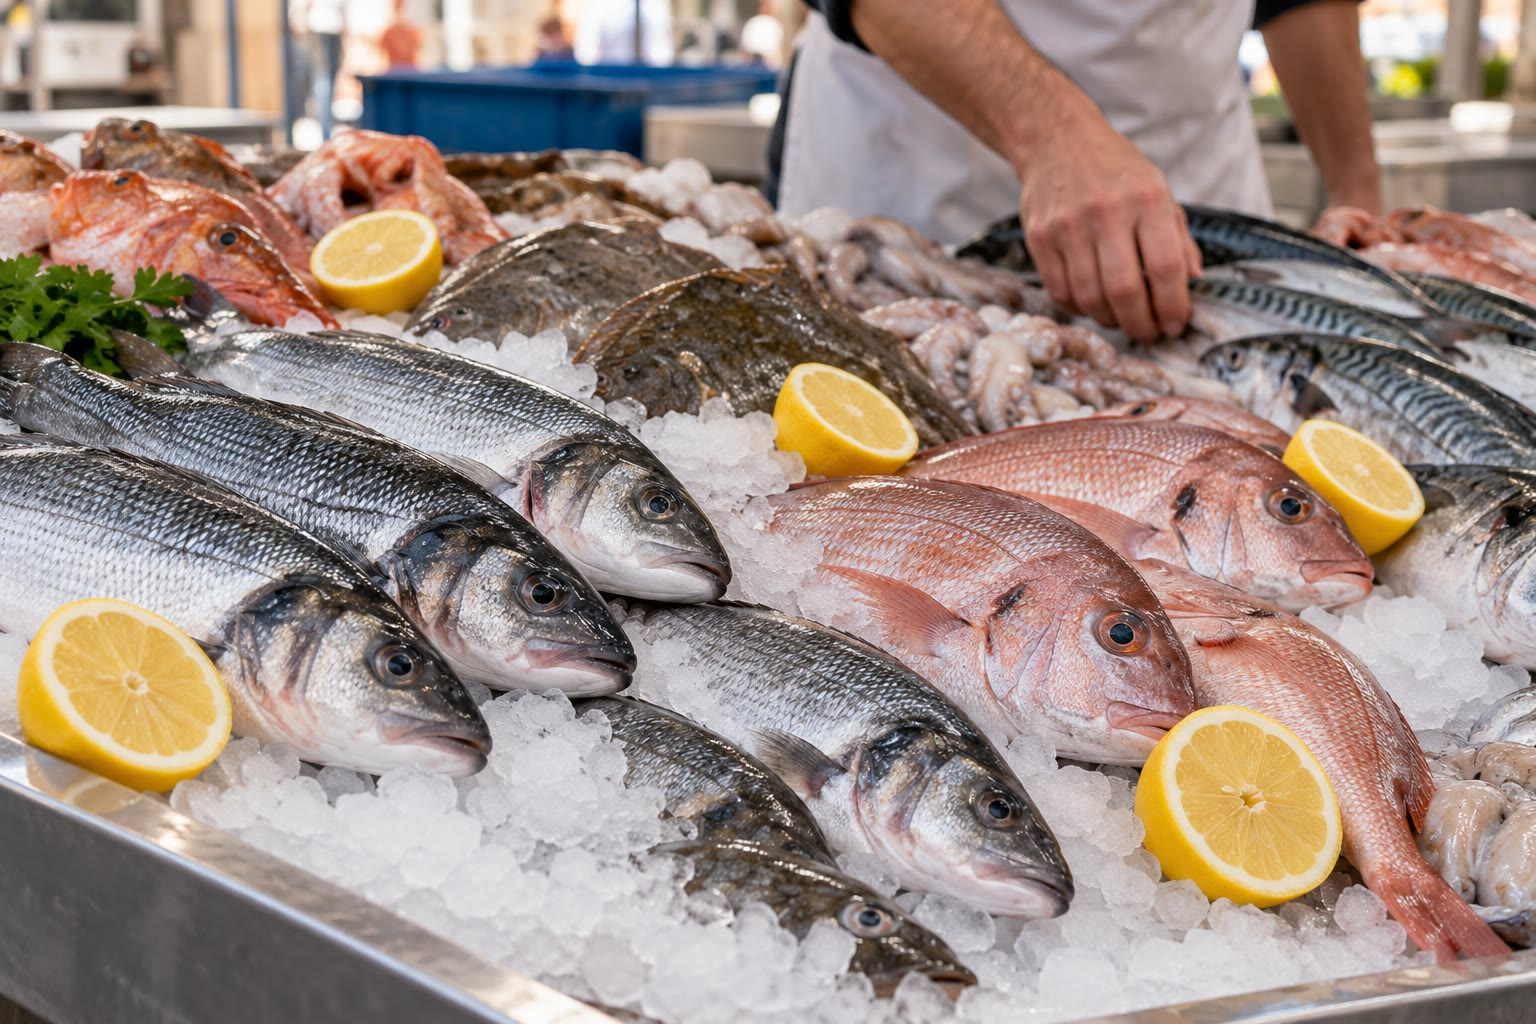
\includegraphics[width=0.6\linewidth]{images/book3/ai/b2-23-fish-stall.jpg}

{\small A fish stall: halved lemons are laid among the fish. Their acid turns the
trimethylamine of the fish into its non-volatile ammonium ion.}
\end{omfigure}

\section{Structure and basicity}

\begin{definition}[Classes of amines]\label{def:b2:amines:class}
An amine is a \emph{primary amine}\index{primary amine} \ce{RNH2}, a \emph{secondary amine}
\index{secondary amine} \ce{R2NH} or a \emph{tertiary amine}\index{tertiary amine}
\ce{R3N} according to the number of carbon groups bound to nitrogen. A \emph{quaternary
ammonium ion}\index{quaternary ammonium ion} \ce{R4N+} has four, and no lone pair.
\end{definition}

The nitrogen of an amine is roughly tetrahedral, the lone pair occupying the fourth
position. A \omterm{def:b2:amines:class}{tertiary amine} with three different groups is chiral in principle but cannot be
resolved: the molecule inverts through a planar arrangement, like an umbrella in the wind,
thousands of millions of times per second at room temperature.

\begin{proposition}[Basicity]\label{prop:b2:amines:basicity}
In water, alkylamines are stronger bases than ammonia ($\mathrm pK_a$ of their ammonium ions
near 10 to 11, against 9.26), arylamines much weaker (anilinium 4.60), and amides hardly
basic at all (protonated ethanamide about $-0.6$).
\end{proposition}

\begin{proof}[Argument]
Alkyl groups push electron density onto nitrogen (inductive effect) and stabilise the
positive charge of the ammonium ion. In water, solvation by hydrogen bonds also matters: an
ion with more \ce{N-H} bonds is better solvated, which is why trimethylammonium (9.80) is a
weaker acid than ammonium but a stronger one than dimethylammonium (10.73). In aniline the lone
pair is delocalised into the ring and is lost on protonation; in an amide it is delocalised
onto the carbonyl oxygen, and protonation occurs, weakly, on oxygen.
% ledger: kb:NH3, pka:methylammonium, pka:dimethylammonium, pka:trimethylammonium, pka:anilinium, pka:ethanamideH
\end{proof}

\begin{omfigure}
\begin{tikzpicture}[font=\small, x=0.85cm]
  \draw[->, thick] (-1.5,0) -- (11.8,0) node[below right] {$\mathrm pK_a$};
  \foreach \x in {0,2,4,6,8,10} \draw (\x,0.1) -- (\x,-0.1) node[below, font=\scriptsize] {\x};
  \foreach \x/\l in {-0.6/{\ce{CH3CONH3+}}, 4.60/{\ce{C6H5NH3+}}} {
    \draw[omDef, thick] (\x,0) -- (\x,0.5);
    \node[font=\scriptsize, anchor=south] at (\x,0.5) {\l};
  }
  \foreach \x/\l/\y/\h in {9.26/{\ce{NH4+} (9.26)}/1.95/1.2, 9.80/{\ce{(CH3)3NH+} (9.80)}/1.45/0.85, 10.66/{\ce{CH3NH3+} (10.66)}/0.95/0.5, 10.73/{\ce{(CH3)2NH2+} (10.73)}/0.45/0.25} {
    \draw[omDef, thick] (\x,0) -- (\x,\h);
    \draw[black!40] (\x,\h) -- (12.2,\y);
    \node[font=\scriptsize, anchor=west] at (12.2,\y) {\l};
  }
  \node[font=\scriptsize, anchor=north west] at (-1.4,-0.5) {weaker bases};
  \node[font=\scriptsize, anchor=north east] at (11.7,-0.5) {stronger bases};
\end{tikzpicture}

{\small $\mathrm pK_a$ of the conjugate acids of some nitrogen bases at
\qty{25}{\degreeCelsius}: the higher it is, the stronger the base.}
% ledger: kb:NH3, pka:methylammonium, pka:dimethylammonium, pka:trimethylammonium, pka:anilinium, pka:ethanamideH
\end{omfigure}

\section{Amines as nucleophiles}

Amines attack halogenoalkanes by bimolecular substitution. The product, a more substituted
amine, is at least as nucleophilic as the starting one and competes for the halogenoalkane:
alkylation of ammonia gives a mixture of primary, secondary and \omterm{def:b2:amines:class}{tertiary amines} and the
quaternary salt.

\begin{proposition}[Polyalkylation]\label{prop:b2:amines:polyalkylation}
Direct alkylation of ammonia or of a \omterm{def:b2:amines:class}{primary amine} gives mixtures; only exhaustive alkylation
to the quaternary ammonium salt is clean.
\end{proposition}

\begin{proof}[Argument]
Each alkylation leaves a lone pair on a nitrogen made more electron-rich by the new alkyl
group; the product reacts with the remaining halogenoalkane at a comparable rate. Only when
nitrogen has no lone pair left, in \ce{R4N+}, does the sequence stop.
\end{proof}

\omterm{def:b2:amines:class}{Primary amines} free of their over-alkylated relatives are made indirectly: by the Gabriel
route (alkylation of the nitrogen of phthalimide, which carries a single acidic hydrogen, then
release of the amine), by reduction of a \omterm{def:b2:amines:nitrile}{nitrile}, of an amide or of a nitro compound, or by
\omterm{def:b2:amines:reductive-amination}{reductive amination} (below).

\section{Imines and enamines}

\begin{definition}[Nucleophilic addition]\label{def:b2:amines:nucleophilic-addition}
A \emph{nucleophilic addition}\index{nucleophilic addition} to a carbonyl group is the attack of
a nucleophile on the carbonyl carbon, which becomes tetrahedral, the \ce{C=O} $\pi$ bond becoming
a lone pair on oxygen.
\end{definition}

\begin{definition}[Hemiaminals, imines and enamines]\label{def:b2:amines:imine}
A \omterm{def:b2:amines:class}{primary amine} adds to an aldehyde or a ketone to give a \emph{hemiaminal}\index{hemiaminal}
(a carbon bearing \ce{OH} and \ce{NHR}); its dehydration gives an \emph{imine}\index{imine}
$\mathrm{R_2C{=}NR'}$. A \omterm{def:b2:amines:class}{secondary amine}, which cannot form a neutral imine, gives after dehydration an
\emph{enamine}\index{enamine} $\mathrm{R_2C{=}CR{-}NR'_2}$, the double bond moving to the adjacent carbon.
\end{definition}

\begin{omfigure}
\setchemfig{atom sep=1.9em}
\schemestart
\chemfig{R_2C=O} \+ \chemfig{H_2N-R'}
\arrow{<=>}
\chemfig{R_2C(-[2]OH)-NH-R'}
\arrow{<=>[\ce{H+}][$-$ \ce{H2O}]}
\chemfig{R_2C=N-R'}
\schemestop
\par\vspace{6pt}

{\small Formation of an \omterm{def:b2:amines:imine}{imine}: \omterm{def:b2:amines:nucleophilic-addition}{nucleophilic addition} of the amine to the carbonyl gives the
\omterm{def:b2:amines:imine}{hemiaminal}; acid catalysis turns its \ce{OH} into a leaving group (\ce{-OH2+}), water leaves and
the nitrogen lone pair forms the \ce{C=N} double bond. Every step is reversible: water in excess
hydrolyses the \omterm{def:b2:amines:imine}{imine} back.}
\end{omfigure}

\begin{proposition}[pH optimum]\label{prop:b2:amines:imine-ph}
\omterm{def:b2:amines:imine}{Imines} form fastest in mildly acidic solution, near pH 4 to 5.
\end{proposition}

\begin{proof}[Argument]
The first step needs the free amine (its lone pair); too acidic a medium protonates the amine
($\mathrm pK_a$ about 10) and removes the nucleophile. The dehydration needs acid to protonate the
hydroxyl group; at high pH it is slow. The rate, the product of the two needs, is largest in
between.
\end{proof}

\begin{definition}[Reductive amination]\label{def:b2:amines:reductive-amination}
A \emph{reductive amination}\index{reductive amination} converts a carbonyl compound and an
amine into a more substituted amine by forming the \omterm{def:b2:amines:imine}{imine} (or iminium ion) and reducing it in the
same pot, usually with sodium cyanoborohydride \ce{NaBH3CN}.
\end{definition}

\begin{proposition}[Selectivity of reductive amination]\label{prop:b2:amines:reductive-amination}
At pH near 6, \ce{NaBH3CN} reduces the iminium ion much faster than the carbonyl compound, so that
the amine is formed without reducing the aldehyde or ketone to an alcohol.
\end{proposition}

\begin{proof}[Argument]
The cyano group makes \ce{BH3CN-} a weak hydride donor, too weak for a neutral carbonyl but
sufficient for a protonated, positively charged iminium ion, a much better electrophile.
\end{proof}

\section{Diazonium salts}

\begin{definition}[Diazonium chemistry]\label{def:b2:amines:diazonium}
A \emph{diazonium ion}\index{diazonium ion} is a cation \ce{R-N+#N}. \emph{Diazotisation}\index{diazotisation}
converts a primary \omterm{def:b2:huckel:aromatic}{aromatic} amine into an aryl diazonium salt with sodium nitrite and a strong acid at
0--\qty{5}{\degreeCelsius}. In a \emph{Sandmeyer reaction}\index{Sandmeyer reaction}, a copper(I) salt
(\ce{CuCl}, \ce{CuBr}, \ce{CuCN}) replaces the diazonium group by Cl, Br or CN with loss of
dinitrogen. In an \emph{azo coupling}\index{azo coupling}, the diazonium ion, a weak electrophile,
attacks an activated \omterm{def:b2:huckel:aromatic}{aromatic} ring to give an azo compound $\mathrm{Ar{-}N{=}N{-}Ar'}$.
\end{definition}

\begin{proposition}[Stability of diazonium ions]\label{prop:b2:amines:diazonium}
Aryl diazonium salts can be kept in cold aqueous solution and used; alkyl \omterm{def:b2:amines:diazonium}{diazonium ions} lose
dinitrogen at once.
\end{proposition}

\begin{proof}[Argument]
Dinitrogen is an excellent leaving group (a very stable molecule, a large entropy gain). For an
alkyl group, loss of \ce{N2} leaves a carbocation, or is attacked directly by water: the ion does
not survive. An aryl cation is very unstable (an empty $\sigma$ orbital in the plane of the ring,
not stabilised by the $\pi$ system), and the \ce{C-N} bond of the aryl \omterm{def:b2:amines:diazonium}{diazonium ion} is
strengthened by conjugation with the ring: at low temperature it persists; warmed, it decomposes,
water replacing the diazonium group by \ce{OH}.
\end{proof}

\begin{omfigure}
\begin{tikzpicture}[font=\small, >={Stealth}]
  \node[cyclenode] (d) at (0,0) {\ce{Ar-N2+}};
  \foreach \a/\t/\c in {90/{\ce{Ar-Cl}}/{\ce{CuCl}}, 150/{\ce{Ar-Br}}/{\ce{CuBr}}, 210/{\ce{Ar-CN}}/{\ce{CuCN}},
                        270/{\ce{Ar-OH}}/{\ce{H2O}, warm}, 330/{\ce{Ar-H}}/{\ce{H3PO2}}, 30/{$\mathrm{Ar{-}N{=}N{-}Ar'}$}/{activated \ce{ArH}}} {
    \node[cyclenode] (p\a) at (\a:2.6) {\t};
    \draw[->, thick] (d) -- (p\a) node[midway, font=\scriptsize, fill=white, inner sep=1pt] {\c};
  }
\end{tikzpicture}

{\small Reactions of an aryl diazonium salt. The \ce{N2+} group is replaced by halogen or
cyanide (Sandmeyer, copper(I) salts), by \ce{OH} (warm water) or by H (hypophosphorous acid), or
kept in an \omterm{def:b2:amines:diazonium}{azo coupling}.}
\end{omfigure}

\begin{method}[Routes through a diazonium salt]\label{met:b2:amines:diazonium-routes}
\begin{enumerate}
  \item Use the amino group (a strong \omterm{def:b2:aromatic-substitution:directing}{ortho/para director}) to place other groups, then convert it
        through the diazonium salt.
  \item Replace it by H to obtain patterns that direct substitution cannot give
        (1,3,5-tribromobenzene from aniline).
  \item Replace it by CN, then hydrolyse to a carboxylic acid: a way to \ce{-COOH} on a ring.
\end{enumerate}
\end{method}

\begin{method}[Making an amine]\label{met:b2:amines:make-amine}
\begin{enumerate}
  \item \omterm{def:b2:amines:class}{Primary amine} on an alkyl chain: Gabriel route, or reduction of a \omterm{def:b2:amines:nitrile}{nitrile} (one carbon
        more than the halogenoalkane used to make it) or of an amide.
  \item Secondary or \omterm{def:b2:amines:class}{tertiary amine}: \omterm{def:b2:amines:reductive-amination}{reductive amination} of the right carbonyl compound with
        the right amine.
  \item \omterm{def:b2:huckel:aromatic}{Aromatic} amine: nitration, then reduction (iron or tin with acid, or \omterm{def:b2:alkene-redox:hydrogenation}{catalytic
        hydrogenation}).
\end{enumerate}
\end{method}

\section{Nitriles}

\begin{definition}[Nitrile]\label{def:b2:amines:nitrile}
A \emph{nitrile}\index{nitrile} is a compound \ce{R-C#N}, made by substitution of a halogenoalkane
by cyanide or by a \omterm{def:b2:amines:diazonium}{Sandmeyer reaction}.
\end{definition}

\begin{proposition}[Reactions of nitriles]\label{prop:b2:amines:nitrile}
A \omterm{def:b2:amines:nitrile}{nitrile} is hydrolysed, in acid or in base, to the amide and then to the carboxylic acid; it is
reduced by lithium aluminium hydride to the \omterm{def:b2:amines:class}{primary amine} \ce{RCH2NH2}; an organomagnesium
reagent adds once to it, and hydrolysis of the \omterm{def:b2:amines:imine}{imine} formed gives a ketone.
\end{proposition}

\begin{proof}[Argument]
The \omterm{def:b2:amines:nitrile}{nitrile} carbon is electrophilic, like a carbonyl carbon: water (activated by acid, or as
hydroxide) adds to it, giving after tautomerism an amide, whose hydrolysis is treated in
\cref{ch:b2:acyl-substitution}. Hydride adds twice. An organomagnesium reagent adds once,
giving an \omterm{def:b2:amines:imine}{imine} anion that does not react further; water then hydrolyses the \omterm{def:b2:amines:imine}{imine} to the ketone.
\end{proof}

\begin{safety}{\ghs[5mm]{GHS03}\,\ghs[5mm]{GHS06}\,\ghs[5mm]{GHS08}\,\ghs[5mm]{GHS09}}
Aniline and \textit{N},\textit{N}-dimethylaniline are toxic by skin contact; sodium nitrite is
toxic and oxidising; sodium cyanoborohydride releases hydrogen cyanide in acid and must be used
in a fume hood. Dry diazonium salts can explode: they are always kept cold, in solution, and used
at once.
% ledger: ghs:aniline, ghs:dimethylaniline, ghs:NaNO2, ghs:NaBH3CN, ghs:sulfanilic-acid
\end{safety}

\section{Exercises}

\begin{exercise}[$\star$]\label{exo:b2:amines:1}
Give the class of: propan-1-amine, \textit{N}-methylethanamine, triethylamine,
tetramethylammonium chloride, aniline.
\end{exercise}

\begin{exercise}[$\star$]\label{exo:b2:amines:2}
Rank by increasing basicity: ammonia, methylamine, aniline, ethanamide.
\end{exercise}

\begin{exercise}[$\star$]\label{exo:b2:amines:3}
Give the \omterm{def:b2:amines:imine}{imine} formed from cyclohexanone and methylamine, and the conditions.
\end{exercise}

\begin{exercise}[$\star$]\label{exo:b2:amines:4}
Starting from benzenediazonium chloride, give the products with \ce{CuBr}, \ce{CuCN}, warm water,
and phenol in base.
\end{exercise}

\begin{exercise}[$\star\star$]\label{exo:b2:amines:5}
Which form of trimethylamine dominates at pH 7, and in what ratio? Explain the lemon, and how an
amine can be extracted from an organic solvent into water.
\end{exercise}

\begin{exercise}[$\star\star$]\label{exo:b2:amines:6}
Give the \omterm{def:b2:amines:imine}{enamine} formed from cyclohexanone and pyrrolidine, and explain why a \omterm{def:b2:amines:class}{secondary amine}
cannot give an \omterm{def:b2:amines:imine}{imine}.
\end{exercise}

\begin{exercise}[$\star\star$]\label{exo:b2:amines:7}
Prepare \textit{N}-benzylpropan-2-amine \ce{C6H5CH2NHCH(CH3)2} by \omterm{def:b2:amines:reductive-amination}{reductive amination}: give two
possible pairs of reagents.
\end{exercise}

\begin{exercise}[$\star\star$]\label{exo:b2:amines:8}
Benzonitrile reacts with ethylmagnesium bromide, then with aqueous acid. Give the product.
\end{exercise}

\begin{exercise}[$\star\star$]\label{exo:b2:amines:9}
Write the Gabriel synthesis of hexan-1-amine and explain why it gives no \omterm{def:b2:amines:class}{secondary amine}.
\end{exercise}

\begin{exercise}[$\star\star\star$]\label{exo:b2:amines:10}
Prepare 1,3,5-tribromobenzene from aniline.
\end{exercise}

\begin{exercise}[$\star\star\star$]\label{exo:b2:amines:11}
Design an azo dye from 4-nitroaniline and phenol: write the \omterm{def:b2:amines:diazonium}{diazotisation}, the coupling (position
and pH), and the product.
\end{exercise}

\begin{exercise}[$\star\star\star$]\label{exo:b2:amines:12}
The quaternary ammonium hydroxide of \textit{N},\textit{N}-dimethylbutan-2-amine, heated, gives
mostly but-1-ene. Explain this Hofmann orientation, opposite to the Zaitsev rule of the Year 1
volume.
\end{exercise}

\section{Problem: Making Methyl Orange}

\begin{problem}[{Weekend problem --- sulfanilic acid and its \omterm{def:b2:amines:diazonium}{diazotisation}, the \omterm{def:b2:amines:diazonium}{azo coupling} with
\textit{N},\textit{N}-dimethylaniline, methyl orange as an indicator, and the yield}]
\label{pb:b2:amines:1}
Data: sulfanilic acid (4-aminobenzenesulfonic acid) \ce{C6H7NO3S}; methyl orange, the sodium salt
\ce{C14H14N3NaO3S}; $\mathrm pK_a$ of the acid form of methyl orange 3.47. Molar masses
(\unit{g/mol}): C 12.011, H 1.008, N 14.007, O 15.999, Na 22.990, S 32.06. Run (exercise data):
\qty{5.00}{g} of sulfanilic acid, yield 80~\%.
% ledger: pka:methylorange, aw:C, aw:H, aw:N, aw:O, aw:Na, aw:S, ghs:sulfanilic-acid, ghs:NaNO2

\medskip
\noindent\textbf{Part I --- Sulfanilic acid and \omterm{def:b2:amines:diazonium}{diazotisation}.}
\begin{enumerate}
  \item Sulfanilic acid exists as a zwitterion. Draw it.
  \item Why is it dissolved in sodium carbonate solution first?
  \item Write the formation of nitrous acid from sodium nitrite and hydrochloric acid.
  \item Write the \omterm{def:b2:amines:diazonium}{diazotisation} of the 4-sulfonatoanilinium ion.
  \item Why is the reaction run at 0--\qty{5}{\degreeCelsius}?
  \item What amount of sodium nitrite is needed for \qty{5.00}{g} of sulfanilic acid?
  \item Why is a slight excess of nitrite tested for, and destroyed?
\end{enumerate}

\medskip
\noindent\textbf{Part II --- The coupling.}
\begin{enumerate}[resume]
  \item Why is \textit{N},\textit{N}-dimethylaniline a good partner?
  \item At which position of its ring does the \omterm{def:b2:amines:diazonium}{diazonium ion} attack, and why?
  \item Write the product (as the sulfonate).
  \item Why is the coupling run in weakly acidic, not strongly acidic, solution?
  \item Why must the solution then be made basic to precipitate the sodium salt?
  \item Why is the \omterm{def:b2:amines:diazonium}{diazonium ion} a weak electrophile, reacting only with activated rings?
\end{enumerate}

\medskip
\noindent\textbf{Part III --- An indicator.}
\begin{enumerate}[resume]
  \item What colour is methyl orange in base, and in acid?
  \item Where does it take a proton?
  \item Over what pH range does its colour change?
  \item Why does the extended conjugated system give a visible colour?
  \item Why does protonation shift the absorption?
\end{enumerate}

\medskip
\noindent\textbf{Part IV --- Yield.}
\begin{enumerate}[resume]
  \item Compute the molar mass of sulfanilic acid.
  \item Compute that of methyl orange (sodium salt).
  \item Compute the amount of sulfanilic acid used.
  \item Compute the theoretical mass of methyl orange.
  \item What losses explain a yield below 100~\%?
  \item State the mass of methyl orange obtained from \qty{5.00}{g} of sulfanilic acid at 80~\%
        yield.
\end{enumerate}
\end{problem}
